%----------------------------------------------------------------------------------------
%	SLIDE 4.
%----------------------------------------------------------------------------------------
\begin{frame}
\frametitle{Using \texttt{physics lists} in Geant4}

\begin{block}{Goal of using \texttt{physics lists}}
	\begin{itemize}
		\item Contains the physical interactions the particles will participate in
		\item With different \texttt{physics list} we'll obtain different results
		\item Important to determine the correct \texttt{physics list} for our similation
	\end{itemize}
\end{block}

\begin{figure}
	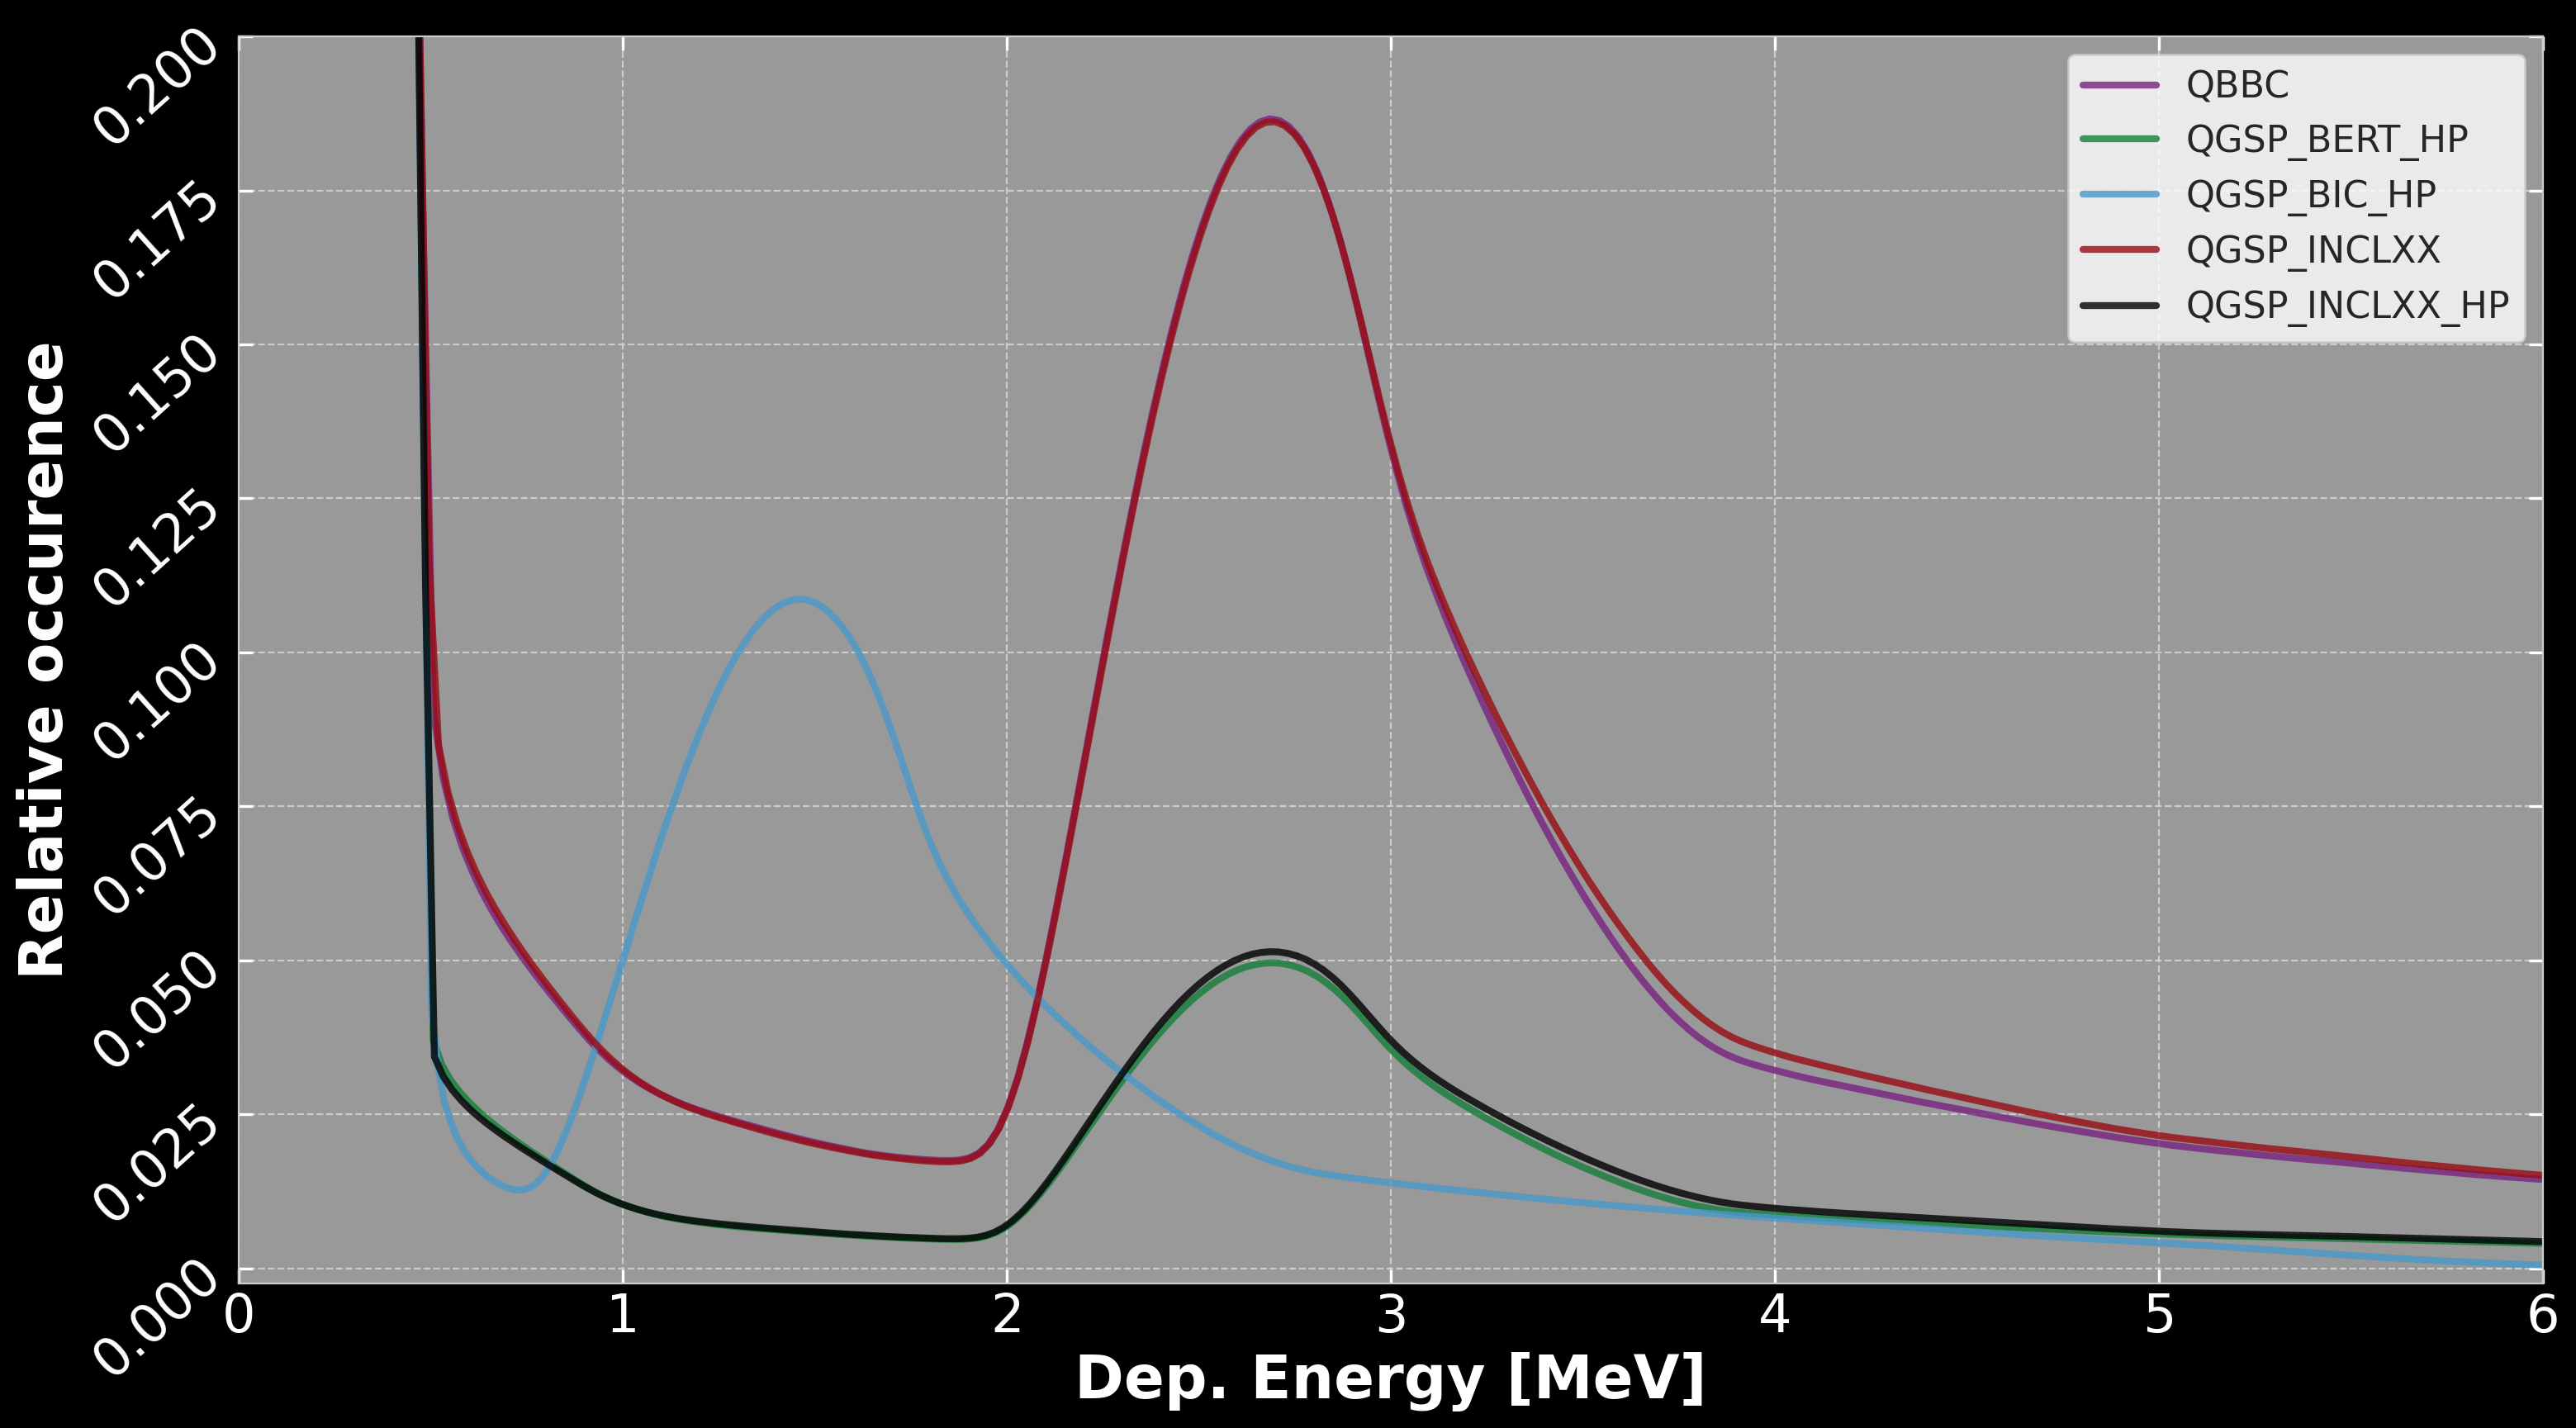
\includegraphics[width=0.75\textwidth]{images/energy_dist_full_concat_E100.png}
\end{figure}

\end{frame}